\section{Query Processing}

We are now at the top two layers of Figure \ref{fig:arch}.


\subsection{Introduction}

To process / parse a query sent from a client (DB application), it is first allocated to a process / thread through a DB engine interface while validating it, checking access control (permissions) and matching it with the query cache. Then, for each uncached query, a query plan (operator tree) is created (possibly rewriting and optimizing the query) and executed while buffers are read from the DB buffer cache or from disk. Finally, the results are sent back to the client.

%TODO oracle / IBM example? images? make tree?

A DB engine is commonly a shared environment with many users running queries concurrently while the engine itself runs its own maintenance procedures. A DB engine is similar to an OS since it has to schedule, orchestrate and mediate access to shared resources.

In a commercial setting, DBs are used programmatically meaning that queries generated by user interfaces are created by application programs. The use of views and query templates affects query processing.


\paragraph{Caching}
In a DB system, it is very likely to receive the same query multiple times and sometimes even in a short time frame. The best way to speed up execution is to reuse results from a previous execution (parsing, optimization, query itself, (intermediate) results\footnote{Query results can be cached in the engine itself or outside of it (intermediate layer, client-side caching, etc.).}, etc.) - everything can be cached! This also works well for data that does not change much (e.g. BLOBS / large data items). As always, consistency problems have to be dealt with.

%TODO oracle / amazon / microsoft example for outside engine caching? more on client caching

\paragraph{Processes vs. Threads}
\begin{itemize}
    \item \textbf{OS Process:} A program execution unit scheduled and managed by the OS with a private and unique address space and its own state.
    \item \textbf{OS Thread:} A program execution unit part of a multi-threaded process that shares its address space and context with other threads from the same process. Scheduled and managed by the kernel.\footnote{Kernel: core program of an OS with complete control over everything in the system. It connects the application software to the hardware (CPU, memory, devices).}
    \item \textbf{Client Process:} Execution unit running on client / application side used to connect to the DB engine.
    \item \textbf{Server Process:} Execution unit running inside the DB engine, used to execute queries on behalf of a client. A query can be processed by several server processes (parallel execution) a.k.a. a pool.
    \item Potentially confusing: the two things above can also be threads in a DB context!
\end{itemize}

With concurrent users, a DB system can be designed to either use a process or a thread for each user session. When using processes, we can take advantage of their isolation and security properties but scalability is limited, context switching is slow (lots of state is maintained) and implementation of parallel query processing is more complex. Furthermore, in a DB context, many data structures are shared across processes (buffer cache, lock table, common memory pools, etc.), which goes against the notion of processes. Most modern systems use threads (shared state and memory facilitates access to common data structures and parallel query processing, lightweight, scalability, etc.) - but more complex management in terms of isolation.

%TODO oracle, postgres example? session definition?

\paragraph{Memory Structures}
Memory needs to be managed carefully since we have many different things running at the same time and shared vs. local memory has to be differentiated. It is common to divide it into regions each with a single purpose.

%TODO oracle example pga (cursor), sga, DB instance, etc.

\paragraph{Cursor}
A pointer to a data structure (table, view, result, etc.) used to navigate the structure - similar to the iterator concept in programming languages. Space needs to be allocated to manage its state (opened, closed, accessed, etc.). When a table is processed, a cursor moves from tuple to tuple. Also used when delivering results to clients - instead of returning a possibly huge table, the cursor to it is returned. %TODO more?


\subsection{Execution Models}

When processing an SQL query, it is parsed into a tree of operators which is the basis for the execution model (see Figure \ref{fig:tree}). The leaves are the tables involved in the query and the root is the final result. Typically, each operator has at most two input from the lower layers (join). Operators can read input / output results one tuple at a time or as a whole - some are even blocking (all operations need to be completed until result can be issued). Each query and each subtree is its own table.

\begin{figure}[h]
	\centering
	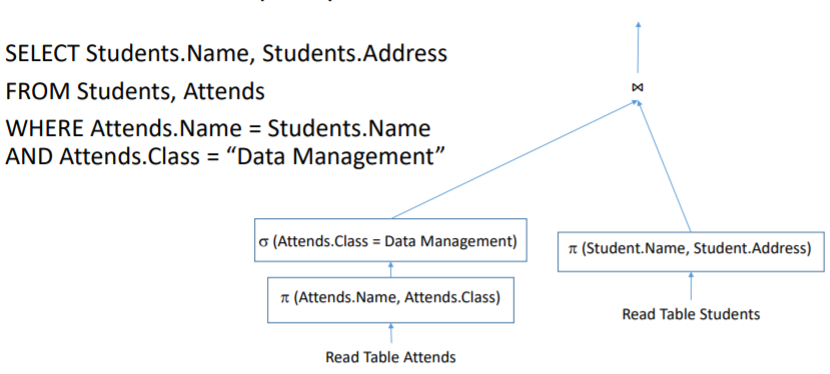
\includegraphics[scale=0.6]{images/3-tree.PNG}
	\caption{Query plan of an example SQL query.}
	\label{fig:tree}
\end{figure}

\paragraph{Pull Mode}
An operator obtains data through a function call to a lower operator (control moves top-down) - data is obtained whenever it is needed. Good for disk-based systems and whenever the data doesn't fit in memory.

\paragraph{Push Mode}
A lower operator sends its result up as soon as it completes processing a tuple / buffer / vector. Higher operators receive results and potentially have to buffer them if they're not ready yet to process them. Can be more efficient than pull mode (hardware / CPU exploitation) but it's more difficult to implement (buffer, synchronization, etc.) - similar to event-based programming. %TODO hardware exploitation


\subsubsection{Single Machine Execution Models}

%TODO operator implementation? if not later

\paragraph{Iterator Model (or Volcano / Pipeline)}
Tuples = data traverse the tree from leaves to the root. Operators iterate over those tuples to process them by using the interface \texttt{Next()}. The execution (control) is top-down (the \texttt{Next()} call initiated at the top trickles down until it can be executed). Once both tables (left and then right) are filled, the nested for-loop is executed. Widely used in disk-based systems and works for all workloads. See Figure \ref{fig:iterator}.

\textbf{Pros:} Generic interface for all operators (great information hiding). Iterators are easy to implement. Supports buffer management strategies. No overhead in terms of main memory. Supports pipelining, parallelism and distribution (with special iterators).

\textbf{Cons:} High overhead of method calls (context switches) and poor instruction cache locality (jumping down and up in the tree calling different functions).

\begin{figure}[h]
	\centering
	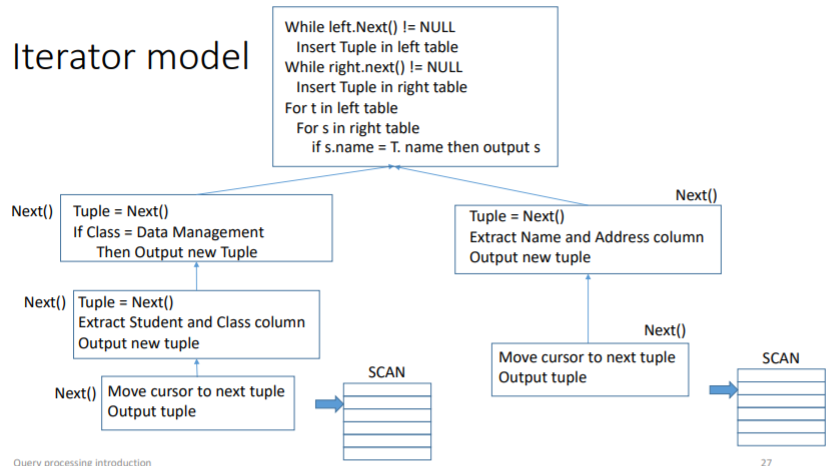
\includegraphics[scale=0.7]{images/3-iterator.PNG}
	\caption{Iterator model of example SQL query (typo: "Name" instead of "Student" in left block).}
	\label{fig:iterator}
\end{figure}

\paragraph{Materialization Model}
Similar to the iterator model but instead of outputting one tuple at a time, each operator outputs its result in a single buffer (each operator is called only once). Much less method calls - less overhead than previous model. Works well in OLTP (queries / transactions process small amounts of data resulting in small buffers that are passed around) - assuming data fits in memory. Not suitable for OLAP since data being passed around can be very large. See Figure \ref{fig:material}.

\begin{figure}[h]
	\centering
	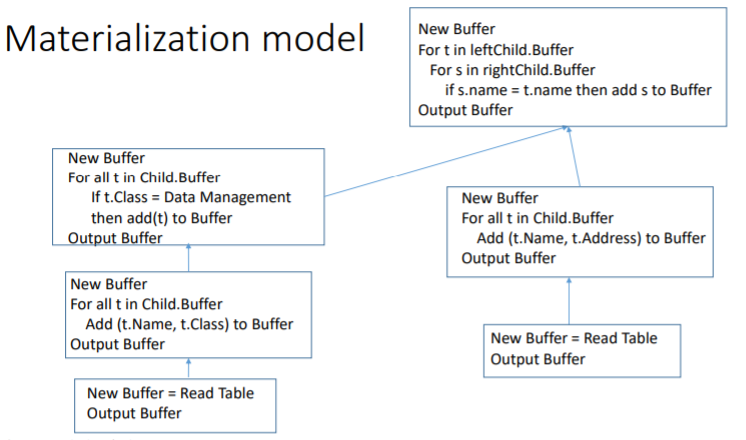
\includegraphics[scale=0.7]{images/3-material.PNG}
	\caption{Materialization model of example SQL query.}
	\label{fig:material}
\end{figure}

\paragraph{Vectorized / Batch Model}
Exploits SIMD / AVX (and column-store) by combining the iterator and materialization model. Data is iterated over with \texttt{Next()} which returns a set of tuples (e.g. entire column) instead of a single one resp. a full buffer. This works best for OLAP systems. %TODO example?


\subsubsection{Parallel Processing Execution Models}

To parallelize a plan or distribute it across several machines, the above models can simply be extended with an \texttt{EXCHANGE} operator. The operator only moves data from one place (e.g. machine) to another - it does not modify data. See Figure \ref{fig:exchange}.

\begin{figure}[h]
	\centering
	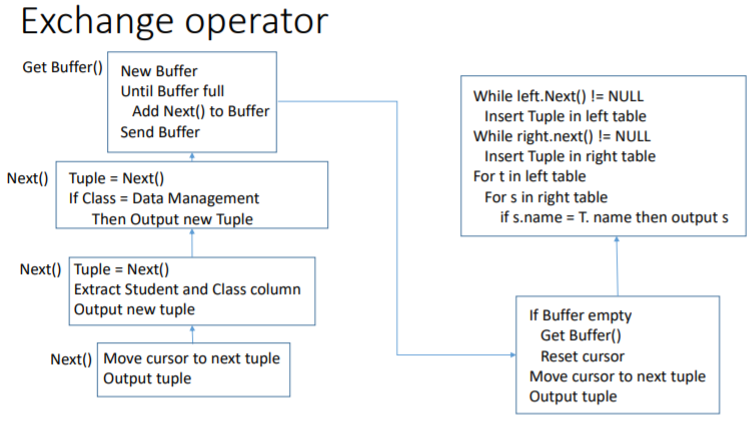
\includegraphics[scale=0.7]{images/3-exchange.PNG}
	\caption{One way to implement an exchange operator (as a driver) shown with example SQL query.}
	\label{fig:exchange}
\end{figure}


\subsection{Query Optimization}

Since SQL is declarative, a DB engine has many options to translate a query into an executable program. After generating possible execution plans for a query, the best one has to be chosen (based on rules or based on estimated cost). A plan is influenced by the access methods for each table (leaves of the query tree), i.e. available indices, predicates, clustered tables (same extent), type of operator implementation, i.e. join implementation, sorted data, and the shape and form of the query tree.

\paragraph{View}
The result set of a stored query on the data (virtual table). A view can be queried just like any other persistent database collection object. Changes applied to the relevant underlying data are perpetuated. A view can me materialized into an actual table and added to the schema (usually done for common operations over the schema). Mainly used to implement logical data independence (create schema different from original one) and access control (access view instead of base tables). %TODO more on why? SQL command

\paragraph{Schema}
A schema is made up of base tables defined at the beginning. It provides the basic organization of the data. Views allow to tailor that logical organization to the needs of particular applications without changing the basic schema. The more complicated a schema is, the more extensive is the use of views. 

%TODO examples: TPC-H, TPC-C/star, snowflake, TPC-DC/snow storm, dimension and fact tables


\subsubsection{Query Rewriting}

After a query has been parsed, it is often rewritten into an equivalent query based on the DB schema and on some heuristics. The rewritten query is then used as input for the query optimization process. 

Rewriting can remove operations to make the query more efficient, can give the optimizer more freedom to operate, can make the query's intent more explicit and can map it to actual base tables and views as needed / for efficiency reasons.

\paragraph{Rewriting Predicates}
A predicate has to be checked for every tuple. The query will run faster if we either reduce the number of comparisons that need to be made and / or if we avoid going several times over the same tuple to check a different predicate. Predicates can be fully transformed or augmented (transitive closure) to decrease the number of comparisons. Augmentation gives the optimizer more options to consider (A=B, B=C - also add A=C; A=B, B$>$100 - also add A$>$100; etc.). Examples in Figures \ref{fig:transormation}, \ref{fig:aug1} and \ref{fig:aug2}.

\begin{figure}[h]
	\centering
	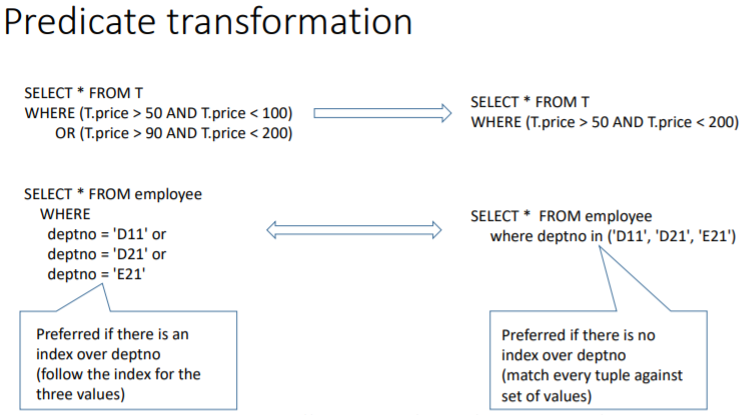
\includegraphics[scale=0.5]{images/3-transformation.PNG}
	\caption{Predicate transformation example.}
	\label{fig:transormation}
\end{figure}

\begin{figure}[h]
	\centering
	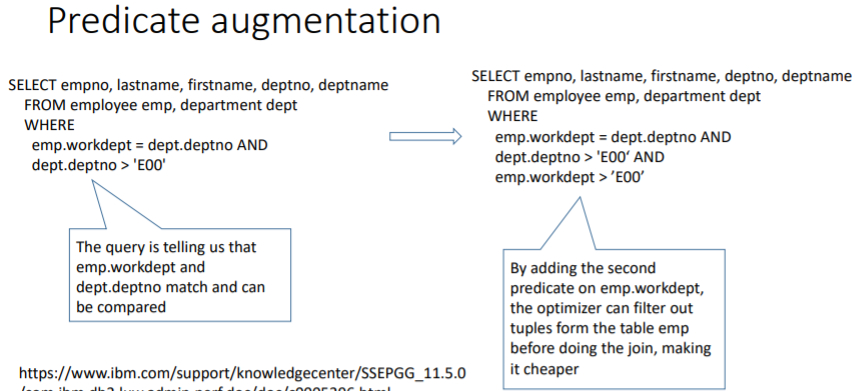
\includegraphics[scale=0.5]{images/3-aug1.PNG}
	\caption{Predicate augmentation example 1.}
	\label{fig:aug1}
\end{figure}

\begin{figure}[h]
	\centering
	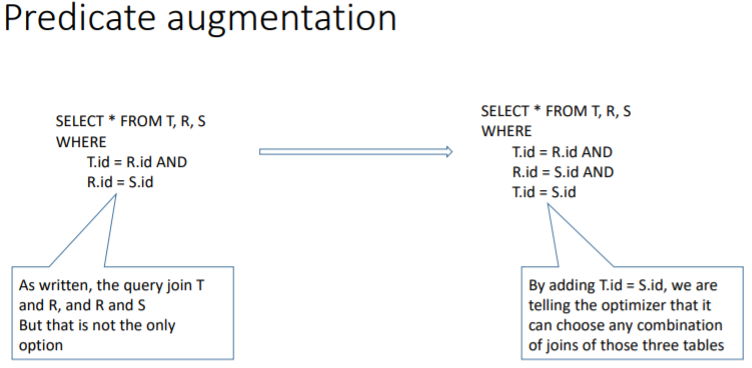
\includegraphics[scale=0.5]{images/3-aug2.PNG}
	\caption{Predicate augmentation example 2.}
	\label{fig:aug2}
\end{figure}

%TODO more examples from slides

\begin{itemize}
    \item Predicate transformation
    \item Predicate augmentation
    \item Arithmetic changes (sum, count, avg)
    \item Predicate pushdown / view folding (view to base table for single pass)
    \item Query unnesting
    \item Materialized views rather than base table %TODO example
    \item Remove distinct if attribute is key
    \item etc. %TODO more "tips"
\end{itemize}


\subsubsection{Rule Based Optimization: Heuristics}

With relational algebra, we can prove equivalence over queries (equivalence rules). This enables query transformations with the guarantee that the results stay the same.

%TODO cheat sheet? examples

\begin{itemize}
    \item Conjunctive selection operations can be deconstructed into a sequence of individual selections.
    \item Selection operations are commutative thus can be applied in a different order.
    \item Selection of a cartesian product = theta join.
    \item Selection of a theta join = theta join with both predicates in conjunction.
    \item Theta / natural joins are commutative.
    \item Natural joins are associative.
    \item Theta joins are associative in a special manner: %TODO
    \item %TODO etcetc
\end{itemize}


\subsubsection{Cost Based Optimization}

To choose the best query plan out of multiple equivalent ones for a query, we might rely on its estimated cost based on many types of information.

\paragraph{Statistics}
Statistics that are constantly collected on tables, indices, buffers and the system itself can be an information source for query optimization (which plan and which operator implementation). We have:

\begin{itemize}
    \item \textbf{Table Statistics:} Number of rows / blocks / etc., average row length, etc.
    \item \textbf{Column Statistics:} Number of distinct values / nulls / etc. (helps to estimate selectivity of a predicate or to decide on join order), data distribution (histogram), etc.
    \item \textbf{Extended Statistics:} Index statistics, number of leaf blocks, levels, clustering factor, etc.
    \item \textbf{System Statistics:} I/O performance and utilization, CPU performance and utilization, etc.
\end{itemize}


\paragraph{Histogram}
Help in cardinality estimation (CE), especially with skewed data. By default, uniform distribution of rows across the distinct values in a column is assumed

%TODO






\subsubsection{Operators}




%TODO





\subsection{Reading Assignments}

\subsubsection{Sort vs. Hash Revisited}

\subsubsection{Query Optimization}

\subsubsection{The State of the Art in Distributed Query Processing}

\subsection{Exercises}

\subsubsection{Query Processing}

\subsubsection{Query Rewriting}

\subsubsection{Query Optimization}

\subsubsection{Cost-Based Optimizer}

\subsubsection{Query Operators}